\section{Temperature of a given day}

Following the first example in the project instructions, the goal of this exercise is to calculate the histogram of the temperature of a given day, the mean temperature of that given day and the standard deviation of the temperature. The function \texttt{tempOnDay} can take as input either the date by month and day, or the day of the year. The histogram gets filled with the temperature of the given day over all years with available data. 

In Figure 1, the resulting histogram for input date (8/23) is presented. The probability of observing a particular temperature on a given day can be calculated by the number of entries in the histogram for the particular temperature divided by the total number of entries.

\begin{figure}[h]
    \centering
    \begin{subfigure}[b]{0.49\textwidth}
    \centering
    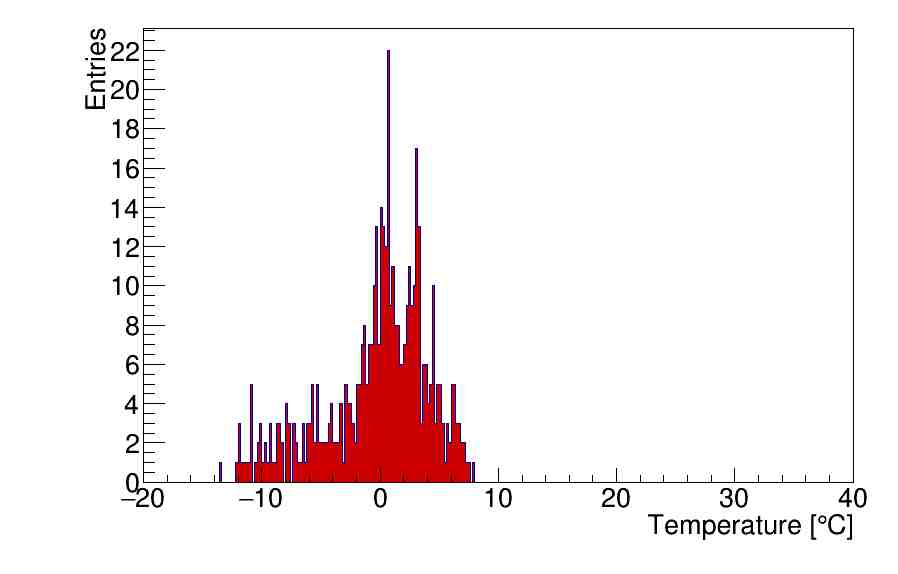
\includegraphics[width=\textwidth]{LU_1_P.jpg}
        \caption{Falsterbo}
    \end{subfigure}
    \hfill
    \begin{subfigure}[b]{0.49\textwidth}
    \centering
    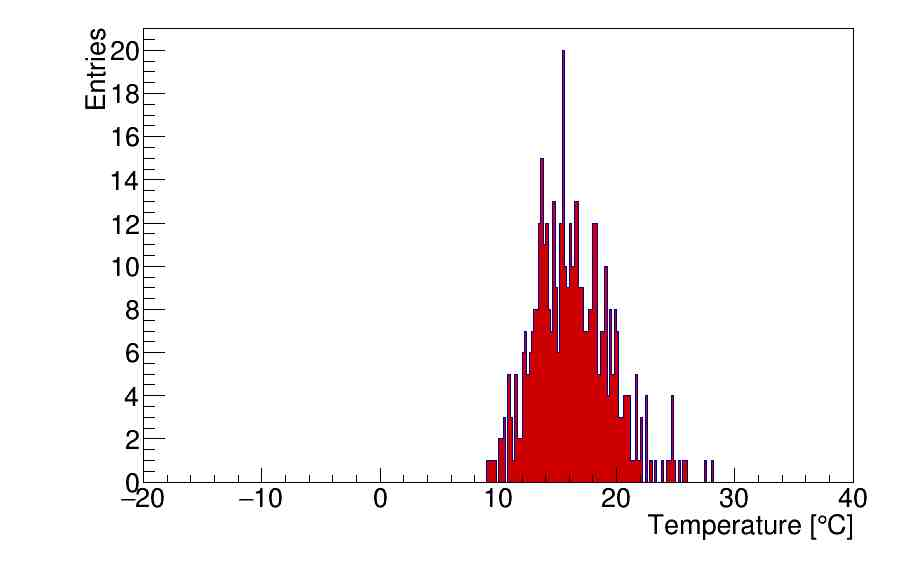
\includegraphics[width=\textwidth]{LU_8_23_P.jpg}
        \caption{Göteborg}
    \end{subfigure}
    
\end{figure}





